\documentclass[../proj1_report.tex]{subfiles}

\begin{document}

\section{Least squares gradient descent}
To test the efficiency of \textit{least_squares_GD} on our dataset, which we standardized, we used cross-validation with five sets to train the hyperparameter $\gamma$.
In figure~\ref{fig:lsgd}, you can observe how fast the cross-validation test error is growing when you change gamma from $0.08$ to $0.09$ but in order to look at a more useful representation of the progression of the error, you can take a look at figure~\ref{fig:lsgd_useful}, which omits the error corresponding to $\gamma = 0.09$.
For the initial weights chosen, they were first all initialized to $0.5$ and seeing the final weights outputted by the program, we modified it to be initialized with values closer to the final weights. Surprisingly, $0.4$ gave a better accuracy result on AICrowd ($69.7\%$) than $0.0$ ($69.3\%$) which was closer to the final weights in general and ouputted a smaller loss.
For the number of iterations, $200$ and $1000$ converged almost to the same loss so to be more efficient, we chose $200$.
Our best submission with \textit{least_squares_GD} had an accuracy of $69.7\%$ and had 
\begin{lstlisting}
max_iters = 200
k_fold = 5
initial_weights = np.array([0.4 for i in range(tX_stdrzed.shape[1])])
gamma = 0.08
\end{lstlisting}

\begin{figure}
    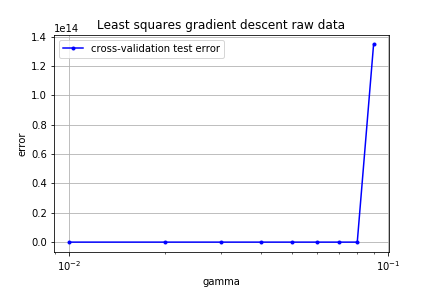
\includegraphics[width= 3, height = 3]{raw_data_least_squares_GD.png}
    \label{fig:lsgd}
\end{figure}

\begin{figure}
    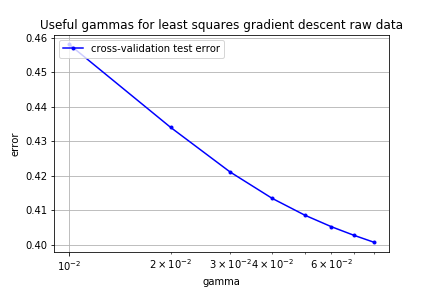
\includegraphics[width= 3, height = 3]{raw_data_least_squares_GD_useful.png}
    \label{fig:lsgd_useful}
\end{figure}



\end{document}